\documentclass[11pt, a4paper]{report}

% --- PACKAGES ---
\usepackage[a4paper, margin=2.5cm]{geometry}
\usepackage{libertinus}
\usepackage{microtype}
\usepackage{graphicx}
\usepackage{xcolor}
\usepackage{hyperref}
\usepackage{titlesec}
\usepackage{tocloft}
\usepackage{booktabs}
\usepackage{enumitem}
\usepackage{fontspec}
\usepackage{listings}
\usepackage{fancyhdr}
\usepackage{amsmath}
\usepackage[table]{xcolor}
\usepackage[backend=biber,style=numeric,sorting=none]{biblatex}
\addbibresource{references.bib}

\directlua{
  luaotfload.add_fallback("monofontemoji", {
      "Apple Color Emoji:mode=harf;"
  })
}

\setmonofont{Libertinus Mono}[RawFeature={fallback=monofontemoji}]

% --- HYPERLINKS STYLING ---
\usepackage{hyperref}
\hypersetup{
  colorlinks=false,
  linkcolor=blue,
  citecolor=blue,
  urlcolor=cyan,
  pdfusetitle
}
\urlstyle{same}

% --- TABLE STYLING ---
\definecolor{TableHeader}{RGB}{30, 34, 40}  % Dark slate
\definecolor{TableRow}{RGB}{245, 245, 245}   % Light gray

\setlist[itemize]{label=--}
\setlength{\parskip}{0.5em}
\setlength{\parindent}{0pt}

% Fix fancyhdr warning about headheight
\setlength{\headheight}{14pt} % or 15pt

% --- CODE STYLING ---
\definecolor{codegreen}{rgb}{0,0.6,0}
\definecolor{codegray}{rgb}{0.5,0.5,0.5}
\definecolor{codepurple}{rgb}{0.58,0,0.82}
\definecolor{backcolour}{rgb}{0.95,0.95,0.92}

\lstdefinestyle{pythonstyle}{
  backgroundcolor=\color{backcolour},
  commentstyle=\color{codegreen},
  keywordstyle=\color{magenta},
  numberstyle=\tiny\color{codegray},
  stringstyle=\color{codepurple},
  basicstyle=\ttfamily\footnotesize,
  breakatwhitespace=false,
  breaklines=true,
  captionpos=b,
  keepspaces=true,
  numbers=left,
  numbersep=5pt,
  showspaces=false,
  showstringspaces=false,
  showtabs=false,
  tabsize=2,
  language=Python
}
\lstset{style=pythonstyle}

% --- HEADER/FOOTER ---
\pagestyle{fancy}
\fancyhf{}
\rhead{\textbf{System Monograph}}
\lhead{Jackson Ferguson}
\cfoot{\thepage}

% --- TITLE FORMATTING ---
\titleformat{\chapter}[display]
{\normalfont\huge\bfseries}{\chaptertitlename\ \thechapter}{20pt}{\Huge}

% =============================================================================
% DOCUMENT START
% =============================================================================
\begin{document}

% --- TITLE PAGE ---
\begin{titlepage}
  \centering
  \vspace*{2cm}

  {\Huge \textbf{From Python to Silicon}}

  \vspace{0.5cm}
  {\Large A Systems Engineering Monograph on \\ Logistics, Power, Analog Synthesis, and Signal Analysis}

  \vspace{1.5cm}

  \textbf{Jackson Ferguson}\\
  \textit{University of Victoria}\\
  \textit{Astrophysics}

  \vspace{2cm}

  \includegraphics[width=0.5\pagewidth]{figures/harmonic_landscape.pdf}

  {\scriptsize\textit{Title graphic generated by the author (Python); source code in the accompanying repository:
  \url{https://github.com/JacksonFergusonDev/systems-audio-lab}.}}

  \vfill

  {\large \today}

\end{titlepage}

% --- ABSTRACT ---
\begin{abstract}
  \noindent This document records a recursive engineering journey: the design and fabrication of the tools required to build a specific device. Identifying a gap between software architecture proficiency and physical implementation, I undertook a project to build an analog guitar pedal (The Red Llama). However, the standard hobbyist workflow proved insufficient for rigorous engineering.

  This monograph details the development of four interdependent systems: (1) \href{https://github.com/JacksonFergusonDev/star-ground}{\textbf{Star Ground}}, a deterministic Python logistics engine for BOM management; (2) A thermal-managed \textbf{Linear Power Supply}; (3) The \textbf{Red Llama} analog overdrive circuit; and (4) A custom \textbf{RP2040 Data Acquisition System} (DAQ) used to spectrally validate the final build.
\end{abstract}

\tableofcontents
\newpage

% =============================================================================
% INTRODUCTION
% =============================================================================
% =============================================================================
% INTRODUCTION
% =============================================================================
% =============================================================================
% INTRODUCTION
% =============================================================================
\chapter{Introduction}

\section{The Systems Engineering Imperative}
In modern computational astrophysics, complex systems are modeled with high precision, yet they remain fundamentally virtual. As an undergraduate specializing in data pipelines and Python, I operate within deterministic environments where logic is absolute and variables are strictly controlled. However, the transition from software architecture to physical implementation reveals a critical discontinuity—the ``Full-Stack Gap.''

In the physical domain, engineering is not merely about logic; it is about managing entropy. Physical systems are subject to stochastic variables—component tolerances, thermal drift, supply chain volatility, and electromagnetic interference—that do not exist in code. This monograph documents a recursive engineering initiative designed to bridge this gap. The primary objective was to fabricate a specific analog device (The Red Llama Overdrive), but the broader pedagogical goal was to apply the rigor of software systems engineering—modularity, regression testing, and version control—to the chaotic reality of hardware fabrication.

\section{Problem Formulation}
The standard hobbyist workflow for electronics fabrication is often characterized by ad-hoc solutions and subjective validation. When analyzed through a systems engineering lens, this approach reveals three critical failure modes that compromise reproducibility and rigorous analysis:

\begin{enumerate}
  \item \textbf{Logistical Entropy:} Unlike software dependencies, which can be resolved instantly via package managers, hardware dependencies are physical and finite. Manual Bill of Materials (BOM) management is nondeterministic and error-prone; a single missing resistor constitutes a critical blocking dependency that can halt a project for weeks.

  \item \textbf{Infrastructure Debt:} Precision audio circuits utilize high-gain amplification stages that are highly susceptible to power supply noise. Standard consumer-grade Switch Mode Power Supplies (SMPS) inherently introduce high-frequency switching ripple \cite{ti_an1950_lownoise_smps}. Relying on generic power infrastructure introduces an uncontrolled variable that aliases into the signal path, invalidating high-fidelity measurements.

  \item \textbf{Subjective Validation:} In audio electronics, verification is often purely qualitative ("it sounds good"). However, from a physics perspective, "tone" is quantifiable as harmonic distortion and frequency response. Without calibrated instrumentation to visualize the transfer function, the engineering process remains blind, relying on trial-and-error rather than empirical data.
\end{enumerate}

\section{Methodology: The Recursive Solution}
To resolve these deficiencies, I elected to engineer the tooling required to build the device, rather than purchasing off-the-shelf solutions. This "recursive" approach ensures that every variable in the signal chain—from the procurement of the silicon to the analysis of the output—is understood and controlled.

This document details the design, fabrication, and integration of four interdependent systems:

\begin{itemize}
  \item \textbf{\href{https://github.com/JacksonFergusonDev/star-ground}{Star Ground} (Logistics):} A Python-based logistics engine that treats hardware BOMs as strict data objects. By parsing PDF documentation into structured JSON data, the system eliminates human error from the procurement process, effectively acting as a "CI/CD pipeline" for physical inventory.

  \item \textbf{Linear Power Regulator (Infrastructure):} A custom, thermal-managed 12V-to-9V linear supply. By utilizing the L7800 series architecture, this subsystem establishes a clean, ripple-free noise floor, ensuring that artifacts observed in the output are generated by the device, not the wall mains.

  \item \textbf{Red Llama Overdrive (Device Under Test):} The primary artifact. This analog circuit utilizes CD4049 CMOS Hex Inverters, originally designed for digital logic, biased into their linear amplification region. This topology is hypothesized to generate soft-clipping saturation characteristics similar to vacuum tube triodes.

  \item \textbf{RP2040 DAQ (Instrumentation):} A custom spectrophotometer and high-speed Analog Front End (AFE). Calibrated against the 60Hz mains frequency, this system enables the empirical verification of the DUT's harmonic content, moving validation from the subjective to the quantitative.
\end{itemize}

\section{Monograph Structure}
The remainder of this document is organized logically following the signal path of the engineering process:
\begin{itemize}
  \item \textbf{Chapter 2} details the software architecture used to manage physical chaos.
  \item \textbf{Chapter 3} outlines the electrical infrastructure required to power the experiment.
  \item \textbf{Chapter 4} describes the fabrication and topology of the analog circuit itself.
  \item \textbf{Chapter 5} explains the design of the digital instrumentation used for analysis.
  \item \textbf{Chapter 6} presents the empirical data, synthesizing the four systems to validate the initial engineering hypotheses.
\end{itemize}

% =============================================================================
% CHAPTER 2: STAR GROUND
% =============================================================================
\chapter{The Logistics Engine (Software)}

\section{Problem Definition: Logistical Entropy}
Before a circuit can be soldered, components must be procured. In the domain of DIY electronics, this is a deceptively complex problem. Bill of Materials (BOM) data is distributed across incompatible formats (PDFs, raw text, forum posts), and inventory management is typically manual.

When managing parts for four concurrent builds, the probability of error approaches unity. A single missing 10-cent resistor creates a shipping bottleneck that halts a project for weeks. I determined that manual transcription of BOMs was an unacceptable source of nondeterministic error.\cite{openbom_bom_pitfalls}

\section{System Architecture: Star Ground}
\textbf{Star Ground} is a Python-based full-stack logistics engine designed to function as the Single Source of Truth for component inventory. In circuit design, a ``Star Ground'' is the point where all signal paths converge to eliminate noise.\cite{nw_star_point_grounding} In this context, the software eliminates the ``noise'' of disorganized supply chains.

\subsection{Design Philosophy: Determinism over AI}
A seemingly obvious solution would be to pass PDF documentation to a Large Language Model (LLM) for parsing. However, for procurement, hallucination is a critical failure mode.\cite{llm_hallucination_survey} If an LLM misidentifies a $100\text{k}\Omega$ resistor as $10\text{k}\Omega$, the hardware will fail.

Therefore, I rejected probabilistic models in favor of a \textbf{Deterministic Regex Engine}. The system uses a Hybrid Strategy for PDF ingestion:
\begin{enumerate}
  \item \textbf{Visual Layout Analysis:} Using \texttt{pdfplumber} to extract table structures based on grid lines.\cite{pdfplumber}
  \item \textbf{Regex Fallback:} A pattern-matching layer that parses raw text when table extraction fails.
  \item \textbf{Snapshot Testing:} We use snapshot-based regression tests that compare the parser's current output against stored ``golden master'' JSON snapshots to detect unintended changes and preserve legacy support. \cite{pytest,pytestregtest}

\end{enumerate}

\section{Algorithmic Logic: Nerd Economics}
The core value of the engine lies in its heuristic inventory buffering. In hardware prototyping, the cost of downtime exceeds the cost of inventory holding. I implemented a ``Yield Management Algorithm'' that adjusts purchase quantities based on component risk profiles.

The engine calculates the Net Need:
\begin{equation}
  \text{Net Need} = \max(0, \text{BOM Qty} - \text{Stock Qty})
\end{equation}

Safety buffers are applied strictly to the deficit:
\begin{itemize}
  \item \textbf{High Risk / Low Cost (Resistors):} $+10$ unit buffer. They are fragile, cheap, and easily lost.
  \item \textbf{Critical Silicon (ICs):} $+1$ unit buffer. Ensures a backup in case of thermal damage during soldering.
  \item \textbf{High Cost (Potentiometers/Switches):} $+0$ buffer.
\end{itemize}

\begin{lstlisting}[caption=Heuristic Buffering Logic]
def calculate_buffer(component_type: str, cost: float) -> int:
    if component_type == "RESISTOR":
        return 10  # Cheap insurance
    elif component_type == "IC" or component_type == "TRANSISTOR":
        return 1   # Protection against ESD/Heat damage
    elif cost > 2.00:
        return 0   # JIT economics
    return 0
\end{lstlisting}

\section{The ``Silicon Sommelier''}
Beyond simple counting, the engine acts as a domain expert system. It utilizes a lookup table to suggest component upgrades based on audio engineering best practices:
\begin{itemize}
  \item \textbf{Op-Amps:} Detects generic \texttt{TL072} chips and suggests Hi-Fi alternatives like \texttt{OPA2134} for lower noise floors.\cite{ti_tl072_datasheet,ti_opa2134_datasheet}
  \item \textbf{Fuzz Logic:} Automatically detects Germanium transistor topologies and flags ``Positive Ground'' warnings.\cite{amplifiedparts_positive_ground,electrosmash_germanium_fuzz}
  \item \textbf{Texture Generation:} Maps clipping diodes to their sonic equivalents based on Forward Voltage ($V_f$).\cite{guitarpedalx_clipping_diodes}
\end{itemize}

\section{Generated Artifacts}
The final output of the pipeline is not just a shopping list, but a structured build guide. The engine generates ``Field Manuals''---PDFs that reorganize the assembly order by component Z-height (Resistors $\to$ Sockets $\to$ Capacitors). This enforces mechanical stability during soldering, ensuring that low-profile components are not obstructed by taller ones.

\section{Validation}
This software was successfully used to procure and manage the inventory for the Red Llama build (Chapter 4) and the Power Regulator (Chapter 3), resulting in zero missing parts and zero excess waste of high-value components.

% =============================================================================
% CHAPTER 3: POWER REGULATOR
% =============================================================================
\chapter{Infrastructure: Linear Power Supply}

\section{Project Motivation}
With the logistics pipeline (Chapter 2) operational, attention turned to the physical infrastructure required to support the Device Under Test (DUT). Audio circuits are notoriously sensitive to power supply noise. Standard consumer-grade ``wall warts'' are typically Switch Mode Power Supplies (SMPS), which operate by rapidly switching a transistor on and off to maintain voltage. This switching frequency often leaks into the audio path, manifesting as high-frequency whine or aliasing artifacts.\cite{ti_an1950_lownoise_smps}

Furthermore, I possessed a surplus of 12V power bricks, but the standard for guitar pedals is 9V Center-Negative. Rather than purchasing a dedicated supply, I elected to engineer a \textbf{Linear Voltage Regulator}. This served a dual purpose: providing a clean, ripple-free power source for the DUT and serving as a low-risk ``Hello World'' for discrete fabrication before attempting the audio circuit.

\section{Theory of Operation}
The circuit relies on the \textbf{L7809CV}, a classic series linear regulator.\cite{st_l7809cv_datasheet} Unlike switching regulators, a linear regulator operates as a variable resistor, effectively ``burning off'' excess voltage as waste heat to maintain a constant output.\cite{st_l7809cv_datasheet} While less efficient than SMPS, the output is practically free of high-frequency ripple, making it ideal for audio applications.

\begin{figure}[htbp]
  \centering
  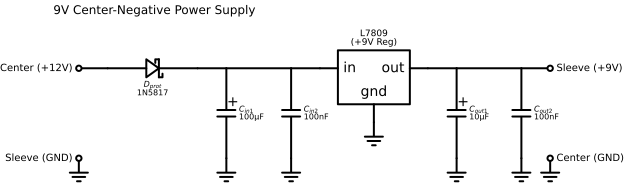
\includegraphics[width=0.8\textwidth]{../power-regulator-12v-to-9v/schematic/exports/power_supply_regulator.pdf}
  \caption{\textbf{Linear Regulator Schematic.} The circuit utilizes a standard L7809 topology with added input/output bulk capacitance and a reverse-bias protection diode ($D_{prot}$) to prevent damage from negative voltage transients.}
  \label{fig:power_schematic}
\end{figure}

\section{Thermal Management Strategy}
The primary engineering constraint in linear regulation is heat dissipation. The power dissipated ($P_d$) is a function of the voltage drop and load current:

\begin{equation}
  P_d = (V_{in} - V_{out}) \times I_{load}
\end{equation}

Given an input of $12\text{V}$ and a target output of $9\text{V}$, the regulator drops $3\text{V}$ across the junction.
\begin{itemize}
  \item \textbf{Scenario A (Red Llama):} The analog DUT draws negligible current ($<10\text{mA}$), resulting in $P_d \approx 0.03\text{W}$.
  \item \textbf{Scenario B (Future Proofing):} Digital pedals (reverbs/delays) can draw upwards of $400\text{mA}$.
\end{itemize}

For Scenario B, the dissipation becomes significant:
\begin{equation}
  P_{max} \approx 3\text{V} \times 0.4\text{A} = 1.2\text{W}
\end{equation}

A standard TO-220 package has a thermal resistance ($\theta_{JA}$) of $\approx 65^\circ \text{C/W}$.\cite{st_l7809cv_datasheet} Without a heatsink, a $1.2\text{W}$ load would result in a temperature rise of:
\begin{equation}
  \Delta T = 1.2\text{W} \times 65^\circ \text{C/W} = 78^\circ \text{C}
\end{equation}
Assuming an ambient temperature of $25^\circ \text{C}$, the silicon junction would reach $103^\circ \text{C}$. While within the absolute maximum ($125^\circ \text{C}$), this is dangerously hot for an enclosed ABS plastic chassis.\cite{st_l7809cv_datasheet}

\subsection{The Solution}
To mitigate this, I implemented a two-stage thermal solution:
\begin{enumerate}
  \item \textbf{Conduction:} A bolt-on aluminum heatsink was attached to the TO-220 package to lower the thermal resistance.
  \item \textbf{Convection:} Ventilation shafts were drilled into the top of the enclosure to establish a convection current, preventing the ABS box from acting as a thermal insulator.
\end{enumerate}

\section{Component Selection}
The Bill of Materials, generated via Star Ground, included specific selections for noise filtering and protection:

\begin{itemize}
  \item \textbf{Input Filtering:} A $100\mu\text{F}$ electrolytic capacitor handles bulk low-frequency ripple from the 12V source, while a parallel $100\text{nF}$ polyester capacitor filters high-frequency transients.\cite{st_l7809cv_datasheet}
  \item \textbf{Reverse Polarity Protection:} A \textbf{1N5817 Schottky Diode} was selected over a standard 1N4001 silicon diode.\cite{diode_1n5817_datasheet,diode_1n4001_datasheet} The Schottky's lower forward voltage drop ($V_f \approx 0.45\text{V}$) preserves more of the input voltage headroom compared to silicon ($V_f \approx 0.7\text{V}$).\cite{diode_1n5817_datasheet,diode_1n4001_datasheet}
\end{itemize}

\begin{table}[htbp]
  \centering
  \small\sffamily
  \renewcommand{\arraystretch}{1.4}
  \setlength{\tabcolsep}{4pt}

  % Alternating row colors: starts at row 2, using TableRow gray and white
  \rowcolors{2}{TableRow}{white}

  \begin{tabular}{@{} l l l l r c r l @{}}
    \toprule
    \rowcolor{TableHeader}
    \textbf{\textcolor{white}{Des.}} &
    \textbf{\textcolor{white}{Value}} &
    \textbf{\textcolor{white}{Component}} &
    \textbf{\textcolor{white}{SKU}} &
    \textbf{\textcolor{white}{Price}} &
    \textbf{\textcolor{white}{Qty}} &
    \textbf{\textcolor{white}{Total}} &
    \textbf{\textcolor{white}{Notes}} \\
    \midrule

    U1 & L7809 & L7809CV-DG Reg 9V 1.5A & A-1597 & \$0.25 & 1 & \$0.25 & TO-220 \\
    $D_{prot}$ & 1N5817 & Schottky Diode 1A 20V & A-159 & \$0.06 & 1 & \$0.06 & Low $V_f$ \\
    $C_{in1}$ & $100\mu\text{F}$ & 35V Radial Electrolytic & A-987 & \$0.03 & 1 & \$0.03 & Bulk In \\
    $C_{out1}$ & $10\mu\text{F}$ & 50V Radial Electrolytic & A-4554 & \$0.02 & 1 & \$0.02 & Bulk Out \\
    $C_{f1,f2}$ & 100nF & 100V 5\% Poly Box & A-564 & \$0.10 & 2 & \$0.20 & HF Filter \\
    J1 & 2.1mm & DC Power Jack (Fem) & A-2237 & \$0.13 & 1 & \$0.13 & Panel Mnt \\
    P1 & 2.1mm & DC Plug (Male) Pigtail & A-6806 & \$0.15 & 1 & \$0.15 & Output \\
    -- & Box & Black Plastic Box 03 & A-2383 & \$2.50 & 1 & \$2.50 & ABS \\
    -- & Heatsink & TO-220 10-Fin 1" & A-1512 & \$0.24 & 1 & \$0.24 & For U1 \\
    -- & M3 & Hex Socket Cap Screw & A-6379 & \$0.10 & 1 & \$0.10 & Mounting \\

    \midrule
    \rowcolor{white}
    \multicolumn{6}{r}{\textbf{PROJECT TOTAL}} & \textbf{\$3.68} & \\
    \bottomrule
  \end{tabular}

  \caption{\textbf{Bill of Materials.} All components sourced from Tayda Electronics to minimize shipping overhead. Prices reflect unit costs at time of purchase.}
  \label{tab:bom_power}
\end{table}

% =============================================================================
% CHAPTER 4: RED LLAMA
% =============================================================================
\chapter{Device Under Test: Red Llama Overdrive}

\section{Circuit Topology}
With the logistics managed (Chapter 2) and the power cleaner (Chapter 3), fabrication began on the primary objective: The \textbf{Red Llama Overdrive}.

This circuit is topologically distinct among guitar pedals. While most overdrives utilize Operational Amplifiers (Op-Amps) with diode clipping in the feedback loop, the Red Llama utilizes the \textbf{CD4049 CMOS Hex Inverter}.\cite{ti_cd4049ub_datasheet}

Originally designed for digital logic (translating 1s and 0s), the CD4049 consists of internal push-pull MOSFET pairs.\cite{ti_cd4049ub_datasheet} By applying negative feedback, the digital gates are forced into a linear amplification region. When driven hard by a guitar signal, the MOSFETs hit the power supply rails, creating a soft, rounded saturation curve that mimics the behavior of vacuum tubes, eventually squaring off into a hard fuzz at maximum gain.

\section{Procurement \& Fabrication}
The build utilized the output artifacts from the \textbf{Star Ground} engine. The ``Field Manual'' PDF dictated the assembly order based on Z-height, ensuring that low-profile resistors were soldered before the taller IC sockets and capacitors. This procedural rigor minimized the mechanical frustration often associated with high-density Perfboard layouts.

\section{Engineering Deviation: The Diode Mod}
While the build largely followed the standard Way Huge Electronics schematic, I introduced a modification to the power section to maximize dynamic range.

The reference design calls for a \textbf{1N4001} silicon diode at position D2 for reverse-polarity protection.\cite{tayda_redllama_schematic} As noted in Chapter 3, silicon diodes exhibit a standard forward voltage drop of $\approx 0.7\text{V}$.\cite{diode_1n4001_datasheet} In a 9V circuit, this drop is non-trivial:

\begin{equation}
  V_{rail} = V_{source} - V_{diode} = 9.0\text{V} - 0.7\text{V} = 8.3\text{V}
\end{equation}

The CD4049's headroom is strictly limited by the supply rails. Losing 0.7V reduces the clean headroom before clipping occurs. To recover this, I substituted the 1N4001 with a \textbf{1N5817 Schottky Diode}.\cite{diode_1n5817_datasheet}

\begin{equation}
  V_{rail(mod)} = 9.0\text{V} - 0.3\text{V} = 8.7\text{V}
\end{equation}

By recovering $\approx 0.4\text{V}$ of supply voltage, the CMOS inverters have slightly more headroom. This translates to increased dynamic range and a cleaner transient response before the onset of saturation.

\section{The Validation Gap}
Upon completion, the device passed the ``Smoke Test'' and produced sound. Subjectively, the tone was rich and harmonically complex. However, as a scientist, subjective listening is insufficient. I required empirical verification of the saturation characteristics.

I did not own an oscilloscope. Rather than buying one, I realized that the surplus \textbf{RP2040} microcontroller I had procured (via the Star Ground logistics run) possessed the theoretical capability to act as a high-speed digitizer.\cite{raspberrypi_rp2040_datasheet} This led to the development of the custom DAQ system detailed in the following chapter.

% =============================================================================
% CHAPTER 5: INSTRUMENTATION (RP2040 DAQ)
% =============================================================================
\chapter{Instrumentation: RP2040 DAQ}

\section{System Architecture}
To validate the saturation behavior of the Red Llama (Chapter 4), I required a Data Acquisition (DAQ) system capable of capturing audio frequencies with high fidelity. The \textbf{RP2040} microcontroller (dual-core ARM Cortex-M0+) was selected as the engine due to its flexible I/O and low cost.\cite{rpi_rp2040_datasheet}

The system operates on a \textbf{"Store-and-Forward"} architecture. Unlike typical streaming applications that push data continuously (and suffer from jitter due to USB packetization), this system prioritizes sample rate stability. It captures a precise burst of data into a pre-allocated ring buffer in RAM, then transmits the binary blob over USB Serial only \textit{after} acquisition is complete.\cite{rpi_rp2040_datasheet} This decouples the strict timing requirements of the sampling loop from the non-deterministic latency of the host workstation.

\section{Analog Front End (AFE) Theory}
The RP2040's internal ADC is limited to a $0\,\text{V}$ to $3.3\,\text{V}$ unipolar range.\cite{rpi_rp2040_datasheet} Direct connection to the Red Llama (which outputs high-amplitude bipolar AC signals) would result in negative voltage clipping and potential silicon latch-up. A "Universal" Signal Conditioning Interface was designed to bridge this gap.

\begin{figure}[htbp]
  \centering
  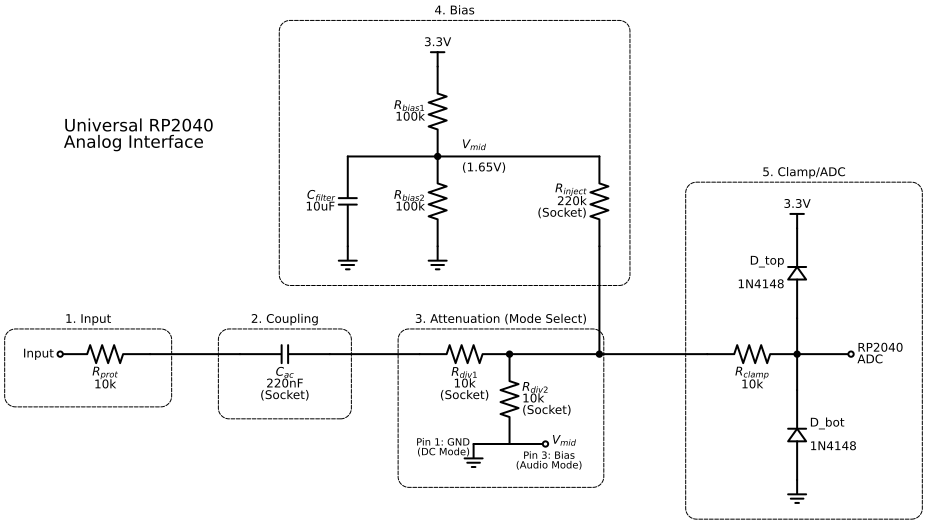
\includegraphics[width=\textwidth]{../oscilloscope-rp2040/schematics/exports/signal_conditioning_universal-blocked.pdf}
  \caption{\textbf{System Schematic.} The signal path flows left-to-right: Protection Stage $\rightarrow$ AC Coupling $\rightarrow$ Attenuation/Bias Network $\rightarrow$ ADC Input.}
  \label{fig:schematic}
\end{figure}

\subsection{Input Protection I}
A series resistor $R_{prot} = 10\,\text{k}\Omega$ is placed immediately at the input jack. This limits the current flowing into the subsequent clamping stage during high-voltage transients or accidental connection to modular synth rails ($\pm 12\,\text{V}$), preventing thermal destruction of the protection diodes.

\subsection{High-Pass Filter (AC Coupling)}
For audio signals, the DC component is blocked using a polyester film capacitor $C_{ac} = 220\,\text{nF}$. The corner frequency ($f_c$) is determined by the input impedance of the subsequent stage.
In \textbf{High-Z / Guitar Mode}, the input impedance is dominated by the bias injection resistor $R_{inject} = 220\,\text{k}\Omega$.

\begin{equation}
  f_c = \frac{1}{2\pi R C} = \frac{1}{2\pi \cdot 220\,\text{k}\Omega \cdot 220\,\text{nF}} \approx 3.29\,\text{Hz}
\end{equation}

This provides a flat frequency response well below the audible floor ($20\,\text{Hz}$).

\subsection{Bias \& Switched Reference Topology}
The RP2040 ADC requires a signal centered at $1.65\,\text{V}$ (half-rail) to read AC waveforms.\cite{rpi_rp2040_datasheet} A stiff voltage divider ($100\,\text{k}\Omega$ pair) filtered by a $10\,\mu$F electrolytic capacitor generates a stable quiet rail ($V_{mid}$).

A \textbf{Switched Reference Topology} is used to solve impedance conflicts via a physical jumper (JP1):
\begin{itemize}
  \item \textbf{Audio Mode:} The jumper connects the bottom of the attenuation network to $V_{mid}$ ($1.65\,\text{V}$). The signal "sees" virtual ground, preserving the gain ratio while biasing the signal center point.
  \item \textbf{DC Mode:} The jumper connects to GND, forming a standard resistive divider for unipolar sensing ($0-5\,\text{V}$ sensors).
\end{itemize}

\subsection{Clamping \& Safety Analysis (Silicon vs. Schottky)}
A critical design decision was the selection of \textbf{1N4148 Silicon Diodes} for rail clamping over standard Schottky diodes.

Standard low-voltage protection often utilizes Schottky diodes (e.g., BAT54) due to their low forward voltage drop ($V_f \approx 0.3\,\text{V}$), which keeps signal excursions strictly within the datasheet absolute maximums ($V_{DD} + 0.5\,\text{V}$).\cite{nexperia_bat54_datasheet} However, Schottky diodes exhibit significant reverse leakage current ($I_R \approx 1\text{--}5\,\mu\text{A}$).\cite{nexperia_bat54_datasheet} Given the High-Z nature of this AFE (specifically the $220\,\text{k}\Omega$ bias injection), a leakage current of just $1\,\mu\text{A}$ would introduce a DC offset error of $V_{err} = 220\,\text{mV}$, significantly reducing dynamic range.

By selecting \textbf{1N4148 Silicon Diodes}, we prioritize precision ($I_R < 25\,\text{nA}$).\cite{generic_1n4148_datasheet} The trade-off is a higher forward voltage ($V_f \approx 0.7\,\text{V}$).\cite{generic_1n4148_datasheet} During an over-voltage event, the clamping node reaches:
\begin{equation}
  V_{clamp} = V_{DD} + V_f = 3.3\,\text{V} + 0.7\,\text{V} = 4.0\,\text{V}
\end{equation}

This exceeds the RP2040 absolute maximum rating of $3.8\,\text{V}$.\cite{rpi_rp2040_datasheet} However, the safety of the device is guaranteed by the current-limiting resistor $R_{clamp}$ ($10\,\text{k}\Omega$). If the external signal forces the node to $4.0\,\text{V}$, the internal ESD diodes of the ADC will begin to conduct at approx $3.8\,\text{V}$. The resulting current injected into the pin is:

\begin{equation}
  I_{inj} = \frac{V_{clamp} - V_{internal}}{R_{clamp}} = \frac{4.0\,\text{V} - 3.8\,\text{V}}{10\,\text{k}\Omega} = 20\,\mu\text{A}
\end{equation}

This injection current of $20\,\mu\text{A}$ is extremely small, and the input is protected primarily by current limiting.

\section{Hardware Configuration}
The board functionality is determined by the presence of socketed components and the position of the 3-pin jumper. This allows the same physical board to serve as a Guitar Interface, Line Level Input, or Sensor Reader.

\begin{table}[htbp]
  \centering
  \small\sffamily
  \renewcommand{\arraystretch}{1.3}
  \rowcolors{2}{TableRow}{white}

  \begin{tabular}{@{} l l l l l @{}}
    \toprule
    \rowcolor{TableHeader}
    \textbf{\textcolor{white}{Mode}} &
    \textbf{\textcolor{white}{Application}} &
    \textbf{\textcolor{white}{Jumper (JP1)}} &
    \textbf{\textcolor{white}{$\mathbf{R_{div1}/R_{div2}}$}} &
    \textbf{\textcolor{white}{$\mathbf{R_{inject}}$}} \\
    \midrule

    Audio (Std)      & Synths, Pedals & Pin 2-3 ($V_{mid}$) & 10k / 10k      & \textit{Empty} \\
    Guitar (High-Z) & Passive Inst.  & Pin 2-3 ($V_{mid}$) & Wire / \textit{Empty} & 220k \\
    DC / Sensor      & 0-5V Signals   & Pin 1-2 (GND)       & 10k / 10k      & \textit{Empty} \\
    \bottomrule
  \end{tabular}

  \caption{Jumper Settings and Component Population Guide}
  \label{tab:config}
\end{table}

\section{Firmware Logic}
The firmware is written in MicroPython to leverage rapid development, but standard Python is too slow for high-speed sampling. To maximize throughput, the critical capture loop uses the \texttt{@micropython.native} decorator.\cite{micropython_speed_python}

\begin{lstlisting}[caption=Native Emitter Capture Loop]
@micropython.native
def capture_burst(adc_obj, buf, size: int):
    # Compiles to ARM Thumb machine code
    for i in range(size):
        buf[i] = adc_obj.read_u16()
\end{lstlisting}

This instructs the compiler to emit ARM Thumb machine code directly.\cite{micropython_speed_python} While the method lookup still incurs overhead, the loop mechanics (increment, compare, jump) become native CPU instructions. This optimization allowed the system to achieve a stable sample rate of $\approx 100\,\text{kSps}$, far exceeding the initial 40\,kSps target.

\section{Calibration: The "Mains Hum" Reference}
Accurate frequency domain analysis requires a precise knowledge of the sampling rate ($F_s$). While the RP2040 hardware clock is stable, the firmware architecture relies on a MicroPython polling loop running on the CPU rather than a DMA-driven hardware timer. Consequently, the effective sample rate is determined by the interpreter's execution overhead, which creates a deterministic but unknown latency.

To resolve this without external signal generators, the system was calibrated using a ubiquitous, high-stability reference standard: the North American Power Grid ($60.00\,\text{Hz}$).

\subsection{Physics of Environmental Coupling}
The calibration signal was acquired by the user touching the input probe tip. This technique exploits the physics of \textbf{capacitive coupling}. The physical system can be modeled as a capacitive voltage divider:
\begin{enumerate}
  \item \textbf{Source ($V_{grid}$):} The 120\,V$_{rms}$ wiring in the walls creates an oscillating electric field ($\omega = 2\pi \cdot 60$).
  \item \textbf{Coupling Impedance ($Z_c$):} The user's body acts as a conductive plate separated from the wiring by a dielectric (air/insulation). This forms a stray capacitance ($C_{stray} \approx 10-100$\,pF).
  \item \textbf{Load Impedance ($Z_{in}$):} The AFE input resistance (approx. $220\,\text{k}\Omega$ in High-Z mode).
\end{enumerate}

The voltage appearing at the ADC ($V_{adc}$) is determined by the ratio of the input impedance to the total path impedance. Given that the reactance of a 50\,pF gap at 60\,Hz is extremely high ($\approx 53\,\text{M}\Omega$), the circuit forms a high-impedance attenuator. However, because the source potential is high ($\approx 170\,\text{V}_{pk}$), even this tiny coupling ratio yields a measurable signal in the millivolt range.

\subsection{Derivation of the Correction Factor}
With the 60\,Hz signal captured, an FFT was performed using the theoretical sample rate ($F_{assumed}$) derived from the loop delay code. The peak analysis revealed a significant discrepancy:
\begin{itemize}
  \item \textbf{Theoretical Peak:} 60.0\,Hz
  \item \textbf{Observed Peak:} 49.9\,Hz
\end{itemize}

This shift indicates that the real-world time steps ($\Delta t$) were larger than calculated (the loop ran slower). Since the frequency axis of an FFT is linear with respect to $F_s$, we can derive a dimensionless scalar correction factor ($\alpha$):

\begin{equation}
  \alpha = \frac{f_{ref}}{f_{meas}} = \frac{60.0}{49.9} \approx 1.2024
\end{equation}

Applying this scalar to the assumed sample rate yields the empirically calibrated rate:

\begin{equation}
  F_{real} = F_{assumed} \times \alpha \approx 97,812\,\text{Hz}
\end{equation}

This ``Golden Constant'' ($F_s \approx 97.8$\,kSps) was hardcoded into the analysis pipeline. Subsequent verification against known audio sources confirmed that this single-point calibration effectively linearized the frequency domain mapping across the full bandwidth.

\section{Final Technical Specifications}
The following specifications reflect the measured performance of the commissioned device.

\begin{table}[htbp]
  \centering
  \small\sffamily
  \renewcommand{\arraystretch}{1.3}
  \rowcolors{2}{TableRow}{white}

  \begin{tabular}{@{} l l @{}}
    \toprule
    \rowcolor{TableHeader}
    \textbf{\textcolor{white}{Parameter}} &
    \textbf{\textcolor{white}{Value / Note}} \\
    \midrule

    \textbf{ADC Resolution}       & 12-bit (Scaled to 16-bit integer) \\
    \textbf{Sample Rate ($F_s$)} & $97.8\,\text{kHz} \pm 0.5\%$ (Calibrated) \\
    \textbf{Bandwidth}           & DC -- 48.9\,kHz (Nyquist Limit) \\
    \textbf{Buffer Depth}        & 16,384 Samples ($\approx 167$\,ms duration) \\
    \textbf{Spectral Resolution} & $\approx 5.9\,\text{Hz}$ per FFT bin \\
    \textbf{Input Range}         & 0--3.3\,V (Unipolar) / $\pm 3.3$\,V (AC Coupled) \\
    \textbf{Noise Floor}         & $<50\,\text{mV}$ (RMS System); $353\,\text{mV}$ (Env. Hum) \\
    \bottomrule
  \end{tabular}

  \caption{Measured System Performance}
  \label{tab:specs}
\end{table}

% =============================================================================
% CHAPTER 6: SYSTEM INTEGRATION & ANALYSIS
% =============================================================================
\chapter{Analysis \& Validation}

\section{Experimental Methodology}
To characterize the Red Llama Overdrive, the device was inserted into the signal chain between a reference source (Electric Guitar, Neck Pickup) and the RP2040 DAQ. The data acquisition pipeline utilized the system's ``Science Mode,'' executing a burst capture of $N=16,384$ samples at a calibrated rate of $F_s \approx 97.8\,\text{kSps}$.

The analysis pipeline was implemented in Python using \texttt{numpy} and \texttt{scipy.signal}.\cite{scipy_signal_tutorial,numpy_fft_fft} Crucially, to mitigate spectral leakage caused by the finite sampling interval, a \textbf{Hann Window} function ($w(n) = 0.5 - 0.5\cos(\frac{2\pi n}{N-1})$) was applied to the raw time-domain buffer prior to the Fast Fourier Transform (FFT).\cite{scipy_fft_tutorial, scipy_hann_window} This preprocessing step ensures that the side-lobes of high-amplitude fundamental frequencies do not obscure the lower-amplitude harmonic distortion products.\cite{harris1978_windows_dft}

\section{DAQ Sensitivity \& Noise Floor}
Before characterizing the Device Under Test (DUT), the instrumentation itself was validated to quantify the available dynamic range. Figure \ref{fig:noise} illustrates the spectral density of the system with the input grounded.

The system exhibits a read noise RMS of $\approx 1.3\text{mV}$. By comparing this noise floor against the saturation limit of the signal chain ($\approx 170\text{mV}_{rms}$ before clipping), we can calculate the effective Signal-to-Noise Ratio (SNR):

\begin{equation}
  \text{SNR}_{dB} = 20 \cdot \log_{10}\left(\frac{V_{signal}}{V_{noise}}\right) = 20 \cdot \log_{10}(129.6) \approx 42.25\,\text{dB}
\end{equation}

This confirms a dynamic range of $>42\,\text{dB}$. Furthermore, the spectrum is remarkably free of the 60Hz mains hum spikes that typically dominate amateur builds, validating the thermal and electrical isolation provided by the \textbf{Linear Power Regulator}.

\begin{figure}[htbp]
  \centering
  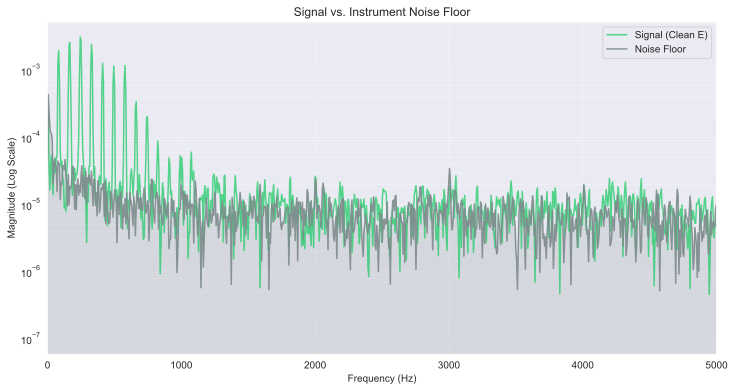
\includegraphics[width=0.9\textwidth]{figures/fig_validation_noise.pdf}
  \caption{\textbf{DAQ Sensitivity Analysis.} The system exhibits a read noise RMS of $\approx 1.3\text{mV}$. Note the clean separation between the signal (green) and the noise floor (gray) below $1\text{kHz}$, yielding an effective SNR of $\approx 42\text{dB}$.}
  \label{fig:noise}
\end{figure}

\section{Gain Structure \& Transfer Characteristic}
The Red Llama operates as a high-gain pre-amplifier. To visualize the amplification factor, the input signal ($\approx 50\text{mV}$) was plotted against the output on a unified voltage scale (Figure \ref{fig:gain}).

The circuit exhibits a measured gain of $\approx 31\text{dB}$ (a voltage ratio of $\approx 36\times$), driving the instrument-level input to near-rail voltages.

\subsection{The Saturation Gradient}
The visual density of the output waveform indicates the physical mechanism of the distortion. Plotting $V_{out}$ as a function of $V_{in}$ reveals the device's \textbf{Transfer Characteristic}.
\begin{itemize}
  \item \textbf{Linear Region:} For small excursions ($|V_{in}| < 50\text{mV}$), the response is ohmic ($R^2 \approx 0.99$).
  \item \textbf{Saturation Region:} As $V_{in}$ approaches the rails ($0\text{V}$ and $3.3\text{V}$), the derivative $dV_{out}/dV_{in}$ approaches zero continuously.
\end{itemize}

Mathematically, this distinguishes the CMOS topology from standard silicon diode clipping. While diodes exhibit a sharp discontinuity ($dV/dt \to \infty$) at the forward voltage threshold ($V_f$), the CMOS inverter behaves as a continuous hyperbolic tangent ($\tanh$) function, resulting in a smoother transition into saturation.

\begin{figure}[htbp]
  \centering
  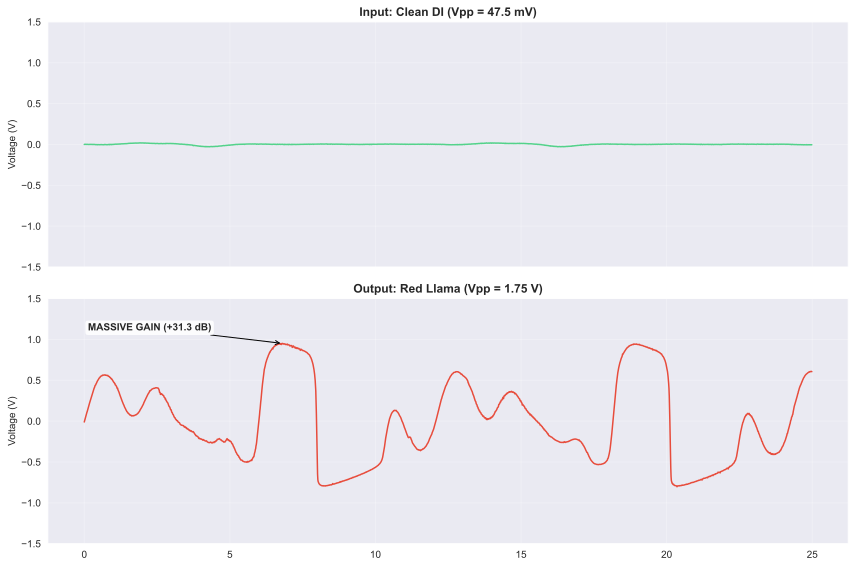
\includegraphics[width=0.9\textwidth]{figures/fig_llama_gain.pdf}
  \caption{\textbf{Gain Stage Characterization.} The circuit provides $\approx 31\text{dB}$ of gain. The squaring of the waveform indicates the onset of heavy saturation, where the MOSFETs collide with the power supply rails.}
  \label{fig:gain}
\end{figure}

\section{Topology \& Harmonic Fingerprint}
The primary engineering hypothesis of this project was that the CD4049 CMOS Hex Inverter, despite being a digital logic chip, behaves analogously to a Vacuum Tube Triode when biased into its linear region. Figure \ref{fig:topology} presents the phase-locked comparison of the Clean vs. Driven signal.

\subsection{Time Domain: The Soft Knee}
As seen in the left panel of Figure \ref{fig:topology}, the waveform peaks exhibit a ``Soft Knee'' compression. This confirms the continuous transfer function described in Section 6.3. The peaks are not sheared off flatly; they are rounded. This preserves the dynamic ``feel'' of the instrument, allowing the player to control the distortion amount via pick attack velocity.

\subsection{Frequency Domain: Even-Order Dominance}
The spectral density analysis (Figure \ref{fig:topology}, Right) reveals the harmonic signature of this topology.
\begin{itemize}
  \item \textbf{Even Harmonics ($2^{nd}, 4^{th}$):} There is a distinct, high-amplitude presence of the 2nd harmonic (the Octave). This asymmetry is mathematically consistent with the single-ended transfer function of vacuum tubes and is responsible for the perceived ``warmth'' of the circuit.
  \item \textbf{Odd Harmonics ($3^{rd}, 5^{th}$):} While present, they do not completely dominate the spectrum as they would in a symmetrical diode-clipping circuit.
\end{itemize}

The clear resolution of these harmonic peaks ($\approx 5.9\,\text{Hz/bin}$) validates the decision to use a custom Hann-windowed FFT pipeline rather than a standard real-time streaming view.

\begin{figure}[htbp]
  \centering
  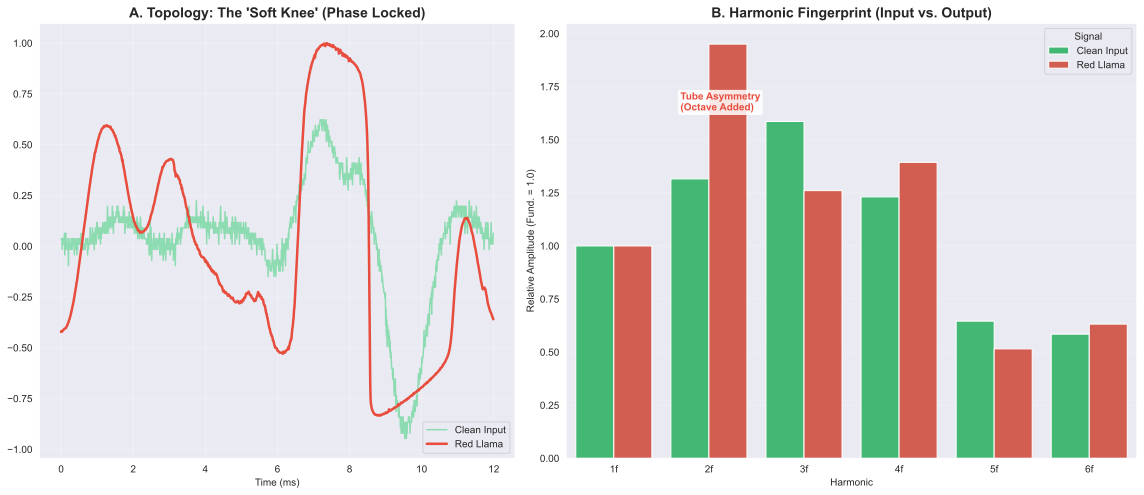
\includegraphics[width=1.0\textwidth]{figures/fig_analysis_topology.pdf}
  \caption{\textbf{Empirical Validation of CMOS Topology.} (A) Phase-locked time domain analysis reveals 'soft knee' compression characteristics distinct from hard diode clipping. (B) Harmonic fingerprinting confirms a dominant 2nd harmonic (octave) and strong even-order series, consistent with the asymmetrical saturation of vacuum tube triodes.}
  \label{fig:topology}
\end{figure}

% =============================================================================
% CHAPTER 7: CONCLUSION
% =============================================================================
\chapter{Conclusion}

\section{Synthesis: The Recursive Engineering Loop}
This monograph documented a deviation from standard hobbyist electronics toward a rigorous systems engineering approach. The project verified that the "Full-Stack Gap" described in Chapter 1 can be bridged not by purchasing better tools, but by engineering them.

The development of the four interdependent systems---Logistics, Infrastructure, Device, and Instrumentation---demonstrated that the principles of software architecture (modularity, determinism, and regression testing)\cite{pytestregtest,pytest} are directly transferable to physical fabrication. The success of the \textbf{Red Llama} build was not a result of manual dexterity, but of the logistical determinism provided by \textbf{Star Ground} and the electrical stability provided by the \textbf{Linear Power Regulator}.

\section{Summary of Empirical Findings}
The analytical phase (Chapter 6) provided quantitative validation of the system's performance. The data supports the following conclusions regarding the \textbf{Red Llama} topology and the custom \textbf{RP2040 DAQ}:

\begin{enumerate}
  \item \textbf{Topological Confirmation (The "Tube" Hypothesis):}
    The transfer characteristic analysis confirmed that the CD4049 CMOS Hex Inverter, when biased into the linear region, exhibits a continuous hyperbolic tangent ($\tanh$) saturation curve.\cite{ti_cd4049ub_datasheet} The absence of derivative discontinuities at the saturation threshold (the "Soft Knee") mathematically distinguishes this circuit from standard silicon diode clipping.

  \item \textbf{Harmonic Fingerprint:}
    Spectral decomposition revealed a dominant 2nd-order harmonic ($f = 2f_0$) and a decaying series of even-order harmonics. This confirms that the CMOS inverter mimics the asymmetrical transfer function of single-ended Class A vacuum tube triodes, validating the psychoacoustic description of the device as "warm" or "amp-like."\cite{sonarworks_distortion_even_odd}

  \item \textbf{Instrumentation Efficacy:}
    The custom RP2040 Data Acquisition System met or exceeded all design requirements.
    \begin{itemize}
      \item \textbf{Bandwidth:} A calibrated sample rate of $97.8\,\text{kSps}$ was achieved, providing a Nyquist frequency of $\approx 48.9\,\text{kHz}$, well beyond the audible spectrum.\cite{nyquist_shannon_sampling}
      \item \textbf{Fidelity:} The system demonstrated a read noise floor of $1.3\text{mV}_{rms}$ and a dynamic range (SNR) of $\approx 42\,\text{dB}$ relative to the saturated signal, proving it is a viable tool for audio frequency analysis.
    \end{itemize}
\end{enumerate}

\section{Future Work \& Optimization}
While the current implementation is functional, specific avenues for optimization have been identified:
\begin{itemize}
  \item \textbf{Automated THD Profiling:} The current analysis relies on burst capture of manual instrument input. A future revision of the DAQ firmware should implement a DAC-driven sine sweep to automatically plot Total Harmonic Distortion (THD) vs. Frequency.\cite{sonarworks_distortion_even_odd}
  \item \textbf{DMA Integration:} Migrating the acquisition loop from CPU-driven polling to Direct Memory Access (DMA) would eliminate jitter and potentially double the sampling rate to $\approx 200\text{--}500\,\text{kSps}$.\cite{rpi_pico_examples_dma_capture,rpi_rp2040_datasheet}
  \item \textbf{Logistics Integration:} The \textbf{Star Ground} engine could be extended to track component "freshness," flagging parts that have been in storage long enough to risk lead oxidation.
\end{itemize}

\section{Phase II: Active Signal Injection (In Progress)}
Current characterization has relied on passive burst capture of organic instrument input. To achieve laboratory-grade transfer function plotting, the project is currently transitioning to an \textbf{Active Signal Injection} phase.

A custom "Host-to-Device" interface is under development, utilizing the host laptop's High-Definition Audio DAC as a signal generator.
\begin{itemize}
  \item \textbf{Hardware Interface:} A custom impedance-matching cable (Aux TRS $\to$ Mono TS) has been fabricated to bridge the consumer line-level output of the host to the high-impedance instrument input of the DUT.
  \item \textbf{Software Generation:} A Python-based Direct Digital Synthesis (DDS) engine has been written to generate precise sine sweeps (20Hz--20kHz) and step functions.
\end{itemize}

This upgrade will allow for the automation of Bode plotting and Total Harmonic Distortion (THD) sweeping in the next revision of this monograph.

\section{Final Remarks}
The \textbf{Red Llama} project stands as a proof-of-concept for the "Systems" approach to maker-electronics. By refusing to treat the supply chain, power delivery, and validation as externalities, the project yielded a device with a verified noise floor and a mathematically characterized distortion profile. This journey confirms that for the modern engineer, the distinction between code and silicon is increasingly arbitrary; both are simply distinct layers of the same stack.

% =============================================================================
% APPENDIX
% =============================================================================
\appendix

\chapter{Source Code}

\section{Firmware: Acquisition Loop}
\textit{MicroPython logic running on the RP2040, handling the high-speed burst capture.}
\lstinputlisting[language=Python, caption=main.py]{../oscilloscope-rp2040/firmware/main.py}

\section{Host: Calibration Algorithm}
\textit{The weighted-average logic used to derive the true sample rate from mains hum (Ref. Chapter 5).}
\lstinputlisting[language=Python, caption=src/calibration.py]{../oscilloscope-rp2040/src/calibration.py}

\section{Host: Signal Processing (DSP)}
\textit{FFT windowing and THD calculation routines (Ref. Chapter 6).}
\lstinputlisting[language=Python, caption=src/dsp.py]{../oscilloscope-rp2040/src/dsp.py}

\section{Host: Function Generator Logic (Phase II)}
\textit{Core logic for the "Laptop-as-Generator" system, capable of generating frequency sweeps for future transfer function analysis.}
\lstinputlisting[language=Python, caption=scripts/signal/play\_sweep.py]{../oscilloscope-rp2040/scripts/signal/play_sweep.py}

% =============================================================================
% REFERENCES
% =============================================================================
\printbibliography[heading=bibintoc,title={References}]

\end{document}